\documentclass[aspectratio=169, 10pt]{beamer}

% ---------- Tema y colores ----------
\usetheme{default}
\usecolortheme{default}
\setbeamertemplate{navigation symbols}{}
\setbeamertemplate{footline}[frame number]
\setbeamertemplate{frametitle continuation}{}

\definecolor{StanfordRed}{RGB}{140,21,21}
\definecolor{LightGray}{RGB}{240,240,240}
\definecolor{AccentGreen}{RGB}{0,130,100}
\definecolor{UCMBlue}{RGB}{4, 171, 226}
\definecolor{UCMNavy}{RGB}{20, 65, 134}

\definecolor{mitblue}{RGB}{20, 65, 134}
\definecolor{mitgray}{RGB}{169, 169, 169}

% Convención de colores: rojo = se adapta, azul = preentrenado y fijo
\definecolor{AdaptRed}{RGB}{200, 40, 40}
\definecolor{FixedBlue}{RGB}{20, 65, 134}

\setbeamercolor{frametitle}{fg=white, bg=UCMBlue}
\setbeamercolor{title}{fg=white}
\setbeamercolor{author}{fg=white}
\setbeamercolor{institute}{fg=white!80}
\setbeamercolor{structure}{fg=UCMBlue}
\setbeamercolor{block title}{bg=UCMBlue!15!white, fg=UCMBlue}
\setbeamercolor{block body}{bg=LightGray}
\setbeamercolor{block title alerted}{bg=StanfordRed!15!white, fg=StanfordRed}
\setbeamercolor{block body alerted}{bg=LightGray}
\setbeamercolor{alerted text}{fg=UCMBlue}

\setbeamerfont{frametitle}{series=\bfseries, size=\large}
\setbeamerfont{title}{series=\bfseries, size=\LARGE}
\setbeamerfont{block title}{series=\bfseries}

% ---------- Paquetes ----------
\usepackage[utf8]{inputenc}
\usepackage[T1]{fontenc}
\usepackage[provide=*,spanish]{babel}
\usepackage{amsmath, amssymb}
\usepackage{graphicx}
\usepackage{tikz}
\usepackage{pgfplots}
\pgfplotsset{compat=1.18}
\usetikzlibrary{arrows, arrows.meta, shapes, shapes.geometric, positioning,
	fit, calc, matrix, chains, mindmap, decorations.pathreplacing,
	backgrounds, shadows, patterns}
\usepackage{booktabs}
\usepackage{xcolor}
\usepackage{multicol}
\usepackage{tcolorbox}
\tcbuselibrary{skins, breakable}
\usepackage{fontawesome5}

% ---------- Comandos útiles ----------
\providecommand{\R}{\mathbb{R}}
\providecommand{\E}{\mathbb{E}}
\newcommand{\frozen}{{\color{FixedBlue}\faLock}}
\newcommand{\tuned}{{\color{AdaptRed}\faFire}}
\newcommand{\ad}[1]{{\color{AdaptRed}#1}}
\newcommand{\fx}[1]{{\color{FixedBlue}#1}}

\newcommand{\formula}[1]{%
	\begin{tcolorbox}[colback=UCMBlue!8, colframe=UCMBlue, arc=4pt,
		boxsep=2pt, left=6pt, right=6pt, top=3pt, bottom=3pt]
		#1
	\end{tcolorbox}
}

% ---------- Portada ----------
\title{\textbf{Transferencia de Aprendizaje}}
\subtitle{Preentrenar, adaptar: finetuning, destilaci\'on, prompting y adaptaci\'on de dominio}
\author{Sergio Hern\'andez, PhD\\ shernandez@ucm.cl}
\institute{
	\begin{tikzpicture}[scale=0.42, every node/.style={transform shape}]
		\foreach \i/\y in {1/0,2/1,3/2}{\node[circle,draw=white,fill=white!20,minimum size=4mm] (i\i) at (0,\y){};}
		\foreach \i/\y in {1/-0.5,2/0.5,3/1.5,4/2.5}{\node[circle,draw=white,fill=white!35,minimum size=4mm] (h\i) at (2,\y){};}
		\foreach \i/\y in {1/0.5,2/1.5}{\node[circle,draw=white,fill=white!50,minimum size=4mm] (o\i) at (4,\y){};}
		\foreach \a in {1,2,3}\foreach \b in {1,2,3,4}{\draw[white,opacity=0.5] (i\a)--(h\b);}
		\foreach \a in {1,2,3,4}\foreach \b in {1,2}{\draw[white,opacity=0.5] (h\a)--(o\b);}
	\end{tikzpicture}
	\\ \textbf{Mag\'ister en Data Science --- Universidad Cat\'olica del Maule}}
\date{}

\begin{document}
% --- Título ---
{
	\setbeamertemplate{background}{
		\begin{tikzpicture}[remember picture, overlay]
			\fill[UCMBlue] (current page.south west) rectangle (current page.north east);
			\fill[UCMBlue!70!black, opacity=0.5]
			(current page.south west) -- ++(0,3) -- ++(18,0) -- cycle;
			\foreach \i in {1,...,40}{
				\fill[white, opacity=0.04]
				({random()*17}, {random()*10}) circle ({random()*0.3});
			}
		\end{tikzpicture}
	}
	\begin{frame}[plain]
		\vspace{1.2cm}
		\titlepage
		\begin{tikzpicture}[remember picture, overlay]
			\node[white, opacity=0.15, font=\fontsize{80}{80}\selectfont]
			at (current page.east) [xshift=-2cm] {$\circlearrowright$};
		\end{tikzpicture}
	\end{frame}
}

% =================================================================
\section{Introducci\'on}

\begin{frame}{Motivaci\'on: el Aprendizaje Profundo es Hambriento de Datos}

	\begin{columns}[T]
		\begin{column}{0.5\textwidth}
			\begin{block}{Redes Profundas}
				\begin{itemize}
					\item Requieren miles (o millones) de ejemplos etiquetados.
					\item Se entrenan \textbf{desde cero} para cada problema.
					\item Etiquetar es caro: m\'edicos, agr\'onomos, expertos.
				\end{itemize}
			\end{block}
		\end{column}

		\begin{column}{0.5\textwidth}
			\begin{block}{Seres Humanos}
				\begin{itemize}
					\item \textbf{One-shot:} aprendemos de un solo ejemplo.
					\item \textbf{Few-shot:} bastan unos pocos ejemplos.
					\item \textbf{Zero-shot:} resolvemos problemas nuevos sin ninguna adaptaci\'on.
				\end{itemize}
			\end{block}
		\end{column}
	\end{columns}

	\vspace{0.4cm}

	\begin{alertblock}{Idea Central}
		La \textbf{transferencia de aprendizaje} reutiliza conocimiento previo para resolver problemas nuevos con pocos datos, en lugar de partir desde cero cada vez.
	\end{alertblock}

\end{frame}

\begin{frame}{Escenario: un Dron Agr\'icola}

	Un dron fue entrenado para clasificar \textbf{trigo vs.\ ma\'iz}. Este a\~no el agricultor cambia de cultivo: ahora debe distinguir \textbf{trigo vs.\ soya}.

	\vspace{0.3cm}

	\begin{center}
		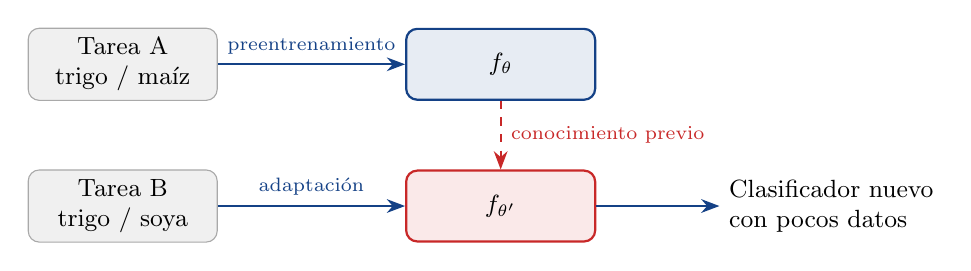
\begin{tikzpicture}[
				box/.style={draw=UCMNavy, thick, rounded corners, fill=UCMNavy!10, minimum width=2.4cm, minimum height=0.9cm, align=center, font=\small},
				data/.style={draw=mitgray, rounded corners, fill=LightGray, minimum width=2.4cm, minimum height=0.9cm, align=center, font=\small},
				arr/.style={-Stealth, thick, UCMNavy}]
			\node[data] (da) at (0,1.2) {Tarea A\\ trigo / ma\'iz};
			\node[box]  (fa) at (4.8,1.2) {$f_\theta$};
			\node[data] (db) at (0,-0.6) {Tarea B\\ trigo / soya};
			\node[box, fill=AdaptRed!10, draw=AdaptRed] (fb) at (4.8,-0.6) {$f_{\theta'}$};
			\node[font=\small, align=left] (out) at (9.0,-0.6) {Clasificador nuevo\\ con pocos datos};

			\draw[arr] (da) -- node[above, font=\scriptsize] {preentrenamiento} (fa);
			\draw[arr] (db) -- node[above, font=\scriptsize] {adaptaci\'on} (fb);
			\draw[arr, dashed, AdaptRed] (fa) -- node[right, font=\scriptsize] {conocimiento previo} (fb);
			\draw[arr] (fb) -- (out);
		\end{tikzpicture}
	\end{center}

	\vspace{0.2cm}

	\begin{block}{Pregunta}
		¿Podemos aprovechar el clasificador existente $f_\theta$ para aprender la nueva tarea m\'as r\'apido y con menos ejemplos?
	\end{block}

\end{frame}

\begin{frame}{Dos Etapas: Preentrenamiento y Adaptaci\'on}

	\begin{columns}[T]
		\begin{column}{0.5\textwidth}
			\begin{block}{1. Preentrenamiento}
				\begin{itemize}
					\item Adquirir \textbf{conocimiento previo}.
					\item Datos masivos y gen\'ericos (ImageNet, LAION, texto web).
					\item Costoso, pero se hace \textbf{una sola vez}.
				\end{itemize}
			\end{block}
		\end{column}

		\begin{column}{0.5\textwidth}
			\begin{block}{2. Adaptaci\'on}
				\begin{itemize}
					\item Aplicar ese conocimiento a una \textbf{tarea nueva}.
					\item Pocos datos, espec\'ificos del dominio.
					\item Barato: minutos u horas.
				\end{itemize}
			\end{block}
		\end{column}
	\end{columns}

	\vspace{0.4cm}

	\begin{block}{¿Qu\'e se puede transferir?}
		\begin{itemize}
			\item \textbf{Pesos} de la red $\to$ finetuning, heads y probes.
			\item \textbf{Salidas} de un modelo maestro $\to$ destilaci\'on.
			\item \textbf{Entradas} modificadas $\to$ prompting, adaptaci\'on de dominio.
			\item \textbf{Datos} sint\'eticos $\to$ modelos generativos.
		\end{itemize}
	\end{block}

\end{frame}

% =================================================================
\section{Finetuning}

\begin{frame}{Finetuning: Ajuste Fino}

	Inicializar el nuevo clasificador con los par\'ametros preentrenados y \textbf{continuar entrenando} en la nueva tarea.

	\vspace{0.3cm}

	\begin{columns}[T]
		\begin{column}{0.48\textwidth}
			\begin{block}{Tres Pasos}
				\begin{enumerate}
					\item Preentrenar $f : \mathcal{X} \to \mathcal{Y}$.
					\item Inicializar $f' = f$.
					\item Ajustar $f' : \mathcal{X}' \to \mathcal{Y}'$ con descenso de gradiente.
				\end{enumerate}
			\end{block}
		\end{column}

		\begin{column}{0.48\textwidth}
			\begin{block}{Algoritmo}
				\small
				\begin{enumerate}
					\item $\theta \leftarrow \arg\min_\theta \sum_{i} \mathcal{L}(f_\theta(x^{(i)}), y^{(i)})$
					\item $\theta' \leftarrow \theta$ \hfill (inicializaci\'on)
					\item $\theta' \leftarrow \arg\min_{\theta'} \sum_{j} \mathcal{L}(f_{\theta'}(x'^{(j)}), y'^{(j)})$
				\end{enumerate}
			\end{block}
		\end{column}
	\end{columns}

	\vspace{0.3cm}

	\begin{alertblock}{Por qu\'e funciona}
		El paso 3 parte de un punto del espacio de par\'ametros que ya codifica caracter\'isticas \'utiles (bordes, texturas, partes de objetos). La optimizaci\'on converge m\'as r\'apido y generaliza mejor con pocos datos.
	\end{alertblock}

\end{frame}

\begin{frame}{Arquitecturas Incompatibles: Reemplazar Capas}

	Si la nueva tarea cambia la dimensi\'on de entrada o salida (p.ej.\ 1000 clases $\to$ 2 clases), no podemos copiar la red completa.

	\vspace{0.3cm}

	\begin{center}
		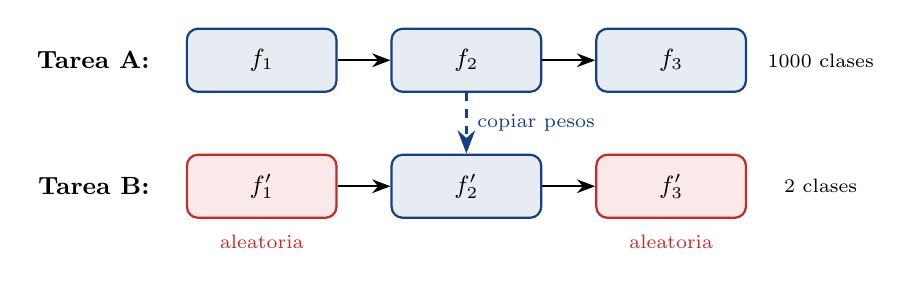
\begin{tikzpicture}[
				lay/.style={draw, thick, rounded corners, minimum width=1.9cm, minimum height=0.8cm, font=\small},
				arr/.style={-Stealth, thick}]
			% Red original
			\node[font=\small\bfseries, anchor=east] at (-0.3,1.3) {Tarea A:};
			\node[lay, draw=FixedBlue, fill=FixedBlue!10] (a1) at (1,1.3) {$f_1$};
			\node[lay, draw=FixedBlue, fill=FixedBlue!10] (a2) at (3.6,1.3) {$f_2$};
			\node[lay, draw=FixedBlue, fill=FixedBlue!10] (a3) at (6.2,1.3) {$f_3$};
			\node[font=\scriptsize] at (8.1,1.3) {1000 clases};
			\draw[arr] (a1) -- (a2); \draw[arr] (a2) -- (a3);

			% Red nueva
			\node[font=\small\bfseries, anchor=east] at (-0.3,-0.3) {Tarea B:};
			\node[lay, draw=AdaptRed, fill=AdaptRed!10] (b1) at (1,-0.3) {$f'_1$};
			\node[lay, draw=FixedBlue, fill=FixedBlue!10] (b2) at (3.6,-0.3) {$f'_2$};
			\node[lay, draw=AdaptRed, fill=AdaptRed!10] (b3) at (6.2,-0.3) {$f'_3$};
			\node[font=\scriptsize] at (8.1,-0.3) {2 clases};
			\draw[arr] (b1) -- (b2); \draw[arr] (b2) -- (b3);

			\draw[-Stealth, dashed, very thick, FixedBlue] (a2) -- node[right, font=\scriptsize] {copiar pesos} (b2);
			\node[font=\scriptsize, AdaptRed] at (1,-1.0) {aleatoria};
			\node[font=\scriptsize, AdaptRed] at (6.2,-1.0) {aleatoria};
		\end{tikzpicture}
	\end{center}

	\formula{
		\[
		f = f_1 \circ f_2 \circ f_3 \qquad \longrightarrow \qquad f' = \ad{f'_1} \circ \fx{f'_2} \circ \ad{f'_3}, \qquad f'_2 \leftarrow f_2
		\]
	}

	Lo usual: conservar el \textbf{cuerpo} (backbone) y reemplazar la \textbf{cabeza} (\'ultima capa).

\end{frame}

\begin{frame}[shrink]{Finetuning de Subpartes de una Red}

	No es necesario ajustar todo: algunos m\'odulos se \textbf{congelan} \frozen{} y otros se \textbf{actualizan} \tuned.

	\vspace{0.2cm}

	\begin{center}
		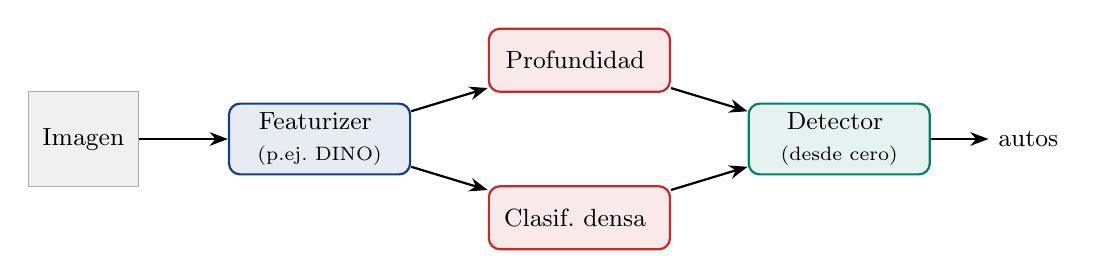
\begin{tikzpicture}[
				mod/.style={draw, thick, rounded corners, minimum width=2.3cm, minimum height=0.8cm, align=center, font=\small},
				arr/.style={-Stealth, thick}]
			\node[draw=mitgray, fill=LightGray, minimum width=1.4cm, minimum height=1.2cm, font=\small] (img) at (0,0) {Imagen};
			\node[mod, draw=FixedBlue, fill=FixedBlue!10] (feat) at (3,0) {Featurizer \frozen\\ \scriptsize (p.ej.\ DINO)};
			\node[mod, draw=AdaptRed, fill=AdaptRed!10] (depth) at (6.3,1) {Profundidad \tuned};
			\node[mod, draw=AdaptRed, fill=AdaptRed!10] (cls) at (6.3,-1) {Clasif.\ densa \tuned};
			\node[mod, draw=AccentGreen, fill=AccentGreen!10] (det) at (9.6,0) {Detector \tuned\\ \scriptsize (desde cero)};
			\node[font=\small] (out) at (12,0) {autos};

			\draw[arr] (img) -- (feat);
			\draw[arr] (feat) -- (depth); \draw[arr] (feat) -- (cls);
			\draw[arr] (depth) -- (det); \draw[arr] (cls) -- (det);
			\draw[arr] (det) -- (out);
		\end{tikzpicture}
	\end{center}

	\vspace{0.2cm}

	\begin{columns}[T]
		\begin{column}{0.5\textwidth}
			\begin{block}{¿Por qu\'e congelar?}
				\small
				\begin{itemize}
					\item \textbf{Componer} modelos que ya resuelven subtareas.
					\item Evitar el \textbf{olvido} del conocimiento previo.
					\item Menos par\'ametros $\Rightarrow$ menos sobreajuste y menos memoria.
				\end{itemize}
			\end{block}
		\end{column}

		\begin{column}{0.5\textwidth}
			\begin{block}{Ajuste de Bajo Rango (LoRA)}
				\small
				En lugar de ajustar $W \in \R^{d \times k}$ completo:
				\[
				W' = \fx{W} + \ad{B A}, \quad B \in \R^{d \times r},\; A \in \R^{r \times k},\; r \ll d,k
				\]
				Ahorra memoria y \textbf{regulariza} la adaptaci\'on.
			\end{block}
		\end{column}
	\end{columns}

\end{frame}

\begin{frame}{Heads y Probes Lineales}

	Un \textbf{probe} es un m\'odulo de lectura liviano $h_\phi$ que toma caracter\'isticas de la red congelada y produce predicciones.

	\formula{
		\[
		\ad{\phi^*} = \arg\min_{\phi} \; \E_{x,y}\Big[\mathcal{L}\big(\ad{h_\phi}(\fx{f_\theta}(x)),\, y\big)\Big], \qquad h_\phi(z) = W z + b
		\]
	}

	\begin{columns}[T]
		\begin{column}{0.48\textwidth}
			\begin{block}{Ventajas}
				\small
				\begin{itemize}
					\item Muy pocos par\'ametros.
					\item Problema convexo: a menudo con \textbf{soluci\'on cerrada} (m\'inimos cuadrados) o regresi\'on log\'istica.
					\item Las caracter\'isticas se calculan una sola vez.
				\end{itemize}
			\end{block}
		\end{column}

		\begin{column}{0.48\textwidth}
			\begin{block}{Doble Prop\'osito}
				\small
				\begin{itemize}
					\item \textbf{Adaptaci\'on:} reutilizar una red para una tarea nueva.
					\item \textbf{An\'alisis:} medir \textit{qu\'e} sabe cada capa. Si un probe lineal predice profundidad desde la capa $\ell$, esa capa codifica profundidad.
				\end{itemize}
			\end{block}
		\end{column}
	\end{columns}

\end{frame}

\begin{frame}{Probes por Capa: ¿D\'onde Est\'a el Conocimiento?}

	\begin{center}
		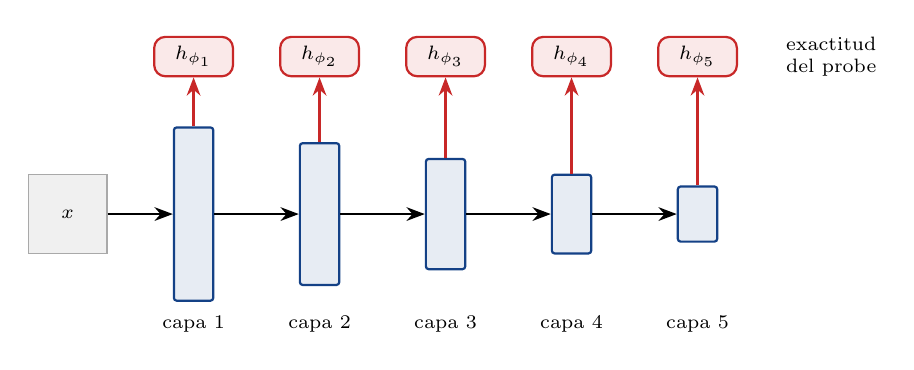
\begin{tikzpicture}[
								prb/.style={draw=AdaptRed, thick, fill=AdaptRed!10, rounded corners, minimum width=1.0cm, minimum height=0.5cm, font=\scriptsize},
				arr/.style={-Stealth, thick}]
			\node[draw=mitgray, fill=LightGray, minimum width=1.0cm, minimum height=1.0cm, font=\scriptsize] (x) at (0,0) {$x$};
			\foreach \i/\h in {1/2.2cm, 2/1.8cm, 3/1.4cm, 4/1.0cm, 5/0.7cm}{
				\node[draw=FixedBlue, thick, fill=FixedBlue!10, minimum width=0.5cm, minimum height=\h, rounded corners=1pt] (l\i) at (1.6*\i,0) {};
				\node[font=\scriptsize] at (1.6*\i,-1.4) {capa \i};
			}
			\draw[arr] (x) -- (l1);
			\foreach \i/\j in {1/2,2/3,3/4,4/5}{\draw[arr] (l\i) -- (l\j);}
			\foreach \i in {1,...,5}{
				\node[prb] (p\i) at (1.6*\i,2.0) {$h_{\phi_\i}$};
				\draw[arr, AdaptRed] (l\i) -- (p\i);
			}
			\node[font=\scriptsize, align=left, anchor=west] at (9,2.0) {exactitud\\ del probe};
			\node[font=\Large] at (9.3,0) {\frozen};
		\end{tikzpicture}
	\end{center}

	\vspace{0.2cm}

	\begin{block}{Patr\'on t\'ipico en CNNs}
		\begin{itemize}
			\item Capas tempranas: bordes, colores, texturas $\to$ \textbf{gen\'ericas}, se transfieren bien.
			\item Capas profundas: partes y conceptos $\to$ \textbf{espec\'ificas} de la tarea de preentrenamiento.
			\item Por eso se reemplazan/ajustan las \'ultimas capas y se reutilizan las primeras.
		\end{itemize}
	\end{block}

\end{frame}

\begin{frame}{Gu\'ia Pr\'actica: ¿Qu\'e Ajustar?}

	\begin{center}
		\renewcommand{\arraystretch}{1.6}
		\begin{tabular}{l|p{4.6cm}|p{4.6cm}}
			\toprule
			& \textbf{Dominio similar} & \textbf{Dominio distinto} \\
			\midrule
			\textbf{Pocos datos} & Probe lineal sobre caracter\'isticas congeladas. & Probe sobre capas intermedias; ajuste cuidadoso (LoRA). \\
			\textbf{Muchos datos} & Finetuning de toda la red con tasa de aprendizaje baja. & Finetuning completo (el preentrenamiento sigue siendo buena inicializaci\'on). \\
			\bottomrule
		\end{tabular}
	\end{center}

	\vspace{0.3cm}

	\begin{alertblock}{Consejos}
		\begin{itemize}
			\item Usar una \textbf{tasa de aprendizaje menor} en el backbone que en la cabeza nueva.
			\item Entrenar primero la cabeza (backbone congelado) y luego descongelar.
			\item Aplicar el mismo preprocesamiento (normalizaci\'on, tama\~no) que en el preentrenamiento.
		\end{itemize}
	\end{alertblock}

\end{frame}

% =================================================================
\section{Aprender de un Maestro}

\begin{frame}{Aprender de un Maestro}

	Hasta ahora aprendemos \textbf{de ejemplos} $(x, y)$. Otra opci\'on: aprender de un \textbf{modelo maestro} $t : \mathcal{X} \to \mathcal{Y}$ ya entrenado.

	\vspace{0.3cm}

	\begin{center}
		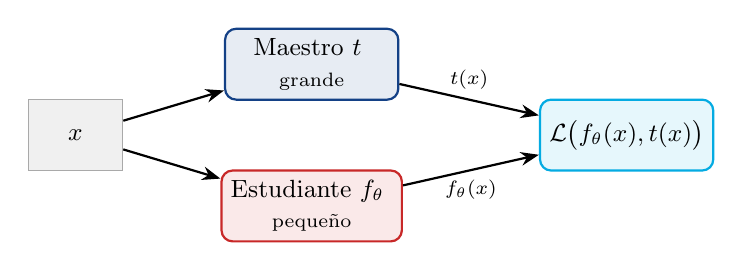
\begin{tikzpicture}[
				box/.style={draw, thick, rounded corners, minimum width=2.2cm, minimum height=0.9cm, align=center, font=\small},
				arr/.style={-Stealth, thick}]
			\node[draw=mitgray, fill=LightGray, minimum width=1.2cm, minimum height=0.9cm, font=\small] (x) at (0,0) {$x$};
			\node[box, draw=FixedBlue, fill=FixedBlue!10] (t) at (3,0.9) {Maestro $t$ \frozen\\ \scriptsize grande};
			\node[box, draw=AdaptRed, fill=AdaptRed!10] (s) at (3,-0.9) {Estudiante $f_\theta$ \tuned\\ \scriptsize peque\~no};
			\node[box, draw=UCMBlue, fill=UCMBlue!10] (L) at (7,0) {$\mathcal{L}\big(f_\theta(x), t(x)\big)$};
			\draw[arr] (x) -- (t); \draw[arr] (x) -- (s);
			\draw[arr] (t) -- node[above, font=\scriptsize] {$t(x)$} (L);
			\draw[arr] (s) -- node[below, font=\scriptsize] {$f_\theta(x)$} (L);
		\end{tikzpicture}
	\end{center}

	\vspace{0.2cm}

	\begin{block}{Dos Modos de Aprender del Maestro}
		\begin{enumerate}
			\item \textbf{Imitar las salidas} del maestro.
			\item \textbf{Igualar las activaciones intermedias} del maestro.
		\end{enumerate}
		El aprendizaje supervisado es un caso particular: el ``maestro'' es el mundo, que s\'olo entrega la etiqueta final.
	\end{block}

\end{frame}

\begin{frame}{Destilaci\'on de Conocimiento}

	\textbf{Destilaci\'on} (Hinton et al., 2015): el estudiante imita la distribuci\'on de probabilidad del maestro.

	\formula{
		\[
		t, f_\theta : \mathcal{X} \to \Delta^{K-1}, \qquad
		\theta^* = \arg\min_\theta \; \E_{x}\Big[\mathcal{L}\big(f_\theta(x),\, t(x)\big)\Big]
		\]
	}

	\begin{columns}[T]
		\begin{column}{0.5\textwidth}
			\begin{block}{Etiqueta Real vs.\ Maestro}
				\small
				Imagen de un gato dom\'estico:
				\begin{itemize}
					\item Etiqueta: \texttt{[gato=1, tigre=0, perro=0]}
					\item Maestro: \texttt{[gato=0.9, tigre=0.1, perro=0]}
				\end{itemize}
				Las \textbf{etiquetas blandas} revelan la estructura de similitud: un gato se parece m\'as a un tigre que a un perro.
			\end{block}
		\end{column}

		\begin{column}{0.5\textwidth}
			\begin{center}
				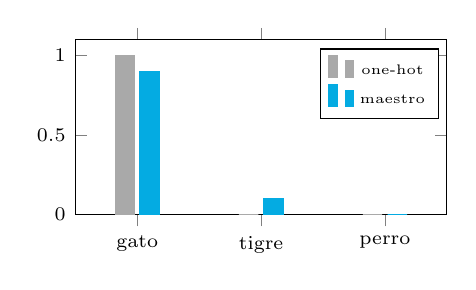
\begin{tikzpicture}
					\begin{axis}[
							ybar, width=6.3cm, height=3.8cm,
							bar width=7pt, ymin=0, ymax=1.1,
							symbolic x coords={gato, tigre, perro},
							xtick=data, tick label style={font=\scriptsize},
							legend style={font=\tiny, at={(0.98,0.95)}, anchor=north east},
							enlarge x limits=0.25]
						\addplot[fill=mitgray, draw=mitgray] coordinates {(gato,1) (tigre,0) (perro,0)};
						\addplot[fill=UCMBlue, draw=UCMBlue] coordinates {(gato,0.9) (tigre,0.1) (perro,0.0)};
						\legend{one-hot, maestro}
					\end{axis}
				\end{tikzpicture}
			\end{center}
		\end{column}
	\end{columns}

\end{frame}

\begin{frame}{Destilaci\'on: Temperatura y P\'erdida}

	Para exponer mejor las probabilidades peque\~nas, se suaviza el softmax con una \textbf{temperatura} $T > 1$:

	\formula{
		\[
		p_k^{(T)} = \frac{\exp(z_k / T)}{\sum_{j} \exp(z_j / T)}, \qquad
		\mathcal{L} = (1-\alpha)\, \mathcal{L}_{CE}\big(y, f_\theta(x)\big) + \alpha\, T^2\, \mathrm{KL}\big(t^{(T)}(x) \,\|\, f^{(T)}_\theta(x)\big)
		\]
	}

	\begin{columns}[T]
		\begin{column}{0.5\textwidth}
			\begin{block}{Por qu\'e funciona}
				\small
				\begin{itemize}
					\item Cada ejemplo aporta $K$ n\'umeros, no s\'olo uno $\Rightarrow$ se\~nal m\'as rica.
					\item Puede acelerar el aprendizaje y requerir menos datos.
					\item No necesita etiquetas: basta con im\'agenes sin anotar.
				\end{itemize}
			\end{block}
		\end{column}

		\begin{column}{0.5\textwidth}
			\begin{block}{Usos}
				\small
				\begin{itemize}
					\item \textbf{Compresi\'on:} modelo grande $\to$ modelo m\'ovil (DistilBERT, TinyViT).
					\item \textbf{Ensembles:} destilar varios modelos en uno.
					\item Hoy el t\'ermino se usa para cualquier m\'etodo estudiante-maestro.
				\end{itemize}
			\end{block}
		\end{column}
	\end{columns}

\end{frame}

% =================================================================
\section{Prompting}

\begin{frame}{Prompting: Adaptar Editando la Entrada}

	\textbf{Prompting}: resolver un problema nuevo \textbf{modificando la entrada}, sin cambiar los par\'ametros del modelo.

	\vspace{0.3cm}

	\begin{columns}[T]
		\begin{column}{0.5\textwidth}
			\begin{block}{En Lenguaje Natural}
				\small
				Se antepone una instrucci\'on al texto:
				\begin{center}
					\texttt{"Responde en franc\'es: ¿qu\'e hora es?"}
				\end{center}
				El mismo modelo resuelve tareas distintas seg\'un el prompt.
			\end{block}
		\end{column}

		\begin{column}{0.5\textwidth}
			\begin{block}{En Visi\'on}
				\small
				\begin{itemize}
					\item \textbf{Prompts de texto} para modelos visi\'on-lenguaje (CLIP: \texttt{"una foto de un \{clase\}"}).
					\item \textbf{Prompts visuales:} agregar p\'ixeles o tokens a la entrada.
					\item Combinaci\'on por concatenaci\'on $\oplus$, suma, u otra mezcla.
				\end{itemize}
			\end{block}
		\end{column}
	\end{columns}

	\vspace{0.3cm}

	\formula{
		\[
		\ad{\epsilon^*} = \arg\min_{\epsilon} \; \E_{x,y}\Big[\mathcal{L}\big(\fx{f_\theta}(x \oplus \ad{\epsilon}),\, y\big)\Big]
		\qquad \text{(s\'olo se aprende el prompt)}
		\]
	}

\end{frame}

\begin{frame}{Prompting en el Espacio de P\'ixeles}

	Se aprende un patr\'on $p$ que se \textbf{suma} a la imagen: $x + p$. T\'ipicamente un \textbf{borde de ruido} optimizado.

	\vspace{0.2cm}

	\begin{columns}[c]
		\begin{column}{0.5\textwidth}
			\begin{center}
				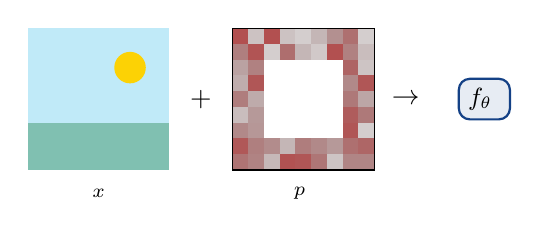
\begin{tikzpicture}
					% Imagen original
					\fill[UCMBlue!25] (0,0) rectangle (1.8,1.8);
					\fill[AccentGreen!50] (0,0) rectangle (1.8,0.6);
					\fill[yellow!70!orange] (1.3,1.3) circle (0.2);
					\node[font=\scriptsize] at (0.9,-0.3) {$x$};
					\node at (2.2,0.9) {$+$};
					% Prompt: borde de ruido
					\begin{scope}[shift={(2.6,0)}]
						\foreach \i in {0,...,8}{
							\foreach \j in {0,...,8}{
								\pgfmathsetmacro{\inner}{(\i>1 && \i<7 && \j>1 && \j<7) ? 1 : 0}
								\ifdim\inner pt=0pt
									\pgfmathsetmacro{\c}{int(20+60*rnd)}
									\fill[AdaptRed!\c!black!\c] (0.2*\i,0.2*\j) rectangle ++(0.2,0.2);
								\fi
							}
						}
						\draw[thin] (0,0) rectangle (1.8,1.8);
						\node[font=\scriptsize] at (0.9,-0.3) {$p$ \tuned};
					\end{scope}
					\node at (4.8,0.9) {$\to$};
					\node[draw=FixedBlue, thick, fill=FixedBlue!10, rounded corners, font=\small] at (5.8,0.9) {$f_\theta$ \frozen};
				\end{tikzpicture}
			\end{center}
		\end{column}

		\begin{column}{0.5\textwidth}
			\formula{
				\[
				\ad{p^*} = \arg\min_{p} \sum_{i} \mathcal{L}\big(f_\theta(x^{(i)} + \ad{p}),\, y^{(i)}\big)
				\]
			}
			\small Un prompt distinto por tarea: clasificaci\'on de escenas, est\'etica, objetos, \ldots
		\end{column}
	\end{columns}

	\vspace{0.3cm}

	\begin{alertblock}{Relaci\'on con Ejemplos Adversarios}
		Matem\'aticamente es casi id\'entico a un ataque adversario (\textit{adversarial reprogramming}), pero el ruido se optimiza para \textbf{mejorar} el desempe\~no en la nueva tarea, no para degradarlo.
	\end{alertblock}

\end{frame}

\begin{frame}{Prompting con Tokens en Vision Transformers}

	En un ViT, se concatenan \textbf{tokens aprendibles} de dimensi\'on $d$ a los tokens de parches.

	\vspace{0.3cm}

	\begin{center}
		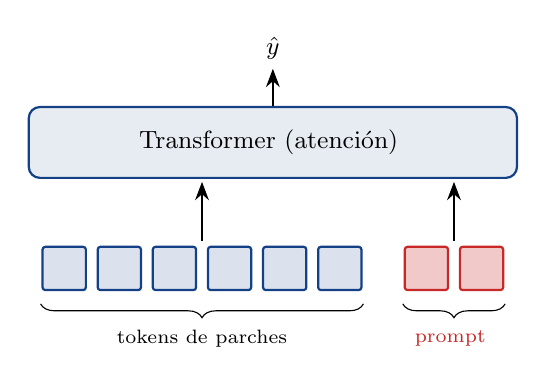
\begin{tikzpicture}[
				tok/.style={draw, thick, minimum width=0.55cm, minimum height=0.55cm, rounded corners=1pt},
				arr/.style={-Stealth, thick}]
			\foreach \i in {0,...,5}{
				\node[tok, draw=FixedBlue, fill=FixedBlue!15] (t\i) at (0.7*\i,0) {};
			}
			\foreach \i in {0,1}{
				\node[tok, draw=AdaptRed, fill=AdaptRed!25] (pr\i) at (4.6+0.7*\i,0) {};
			}
			\draw[decorate, decoration={brace, mirror, amplitude=5pt}] (-0.3,-0.45) -- (3.8,-0.45) node[midway, below=6pt, font=\scriptsize] {tokens de parches};
			\draw[decorate, decoration={brace, mirror, amplitude=5pt}] (4.3,-0.45) -- (5.6,-0.45) node[midway, below=6pt, font=\scriptsize, AdaptRed] {prompt \tuned};

			\node[draw=FixedBlue, thick, fill=FixedBlue!10, rounded corners, minimum width=6.2cm, minimum height=0.9cm, font=\small] (enc) at (2.65,1.6) {Transformer (atenci\'on) \frozen};
			\draw[arr] (1.75,0.35) -- (1.75,1.1);
			\draw[arr] (4.95,0.35) -- (4.95,1.1);
			\node[font=\small] (y) at (2.65,2.8) {$\hat{y}$};
			\draw[arr] (enc) -- (y);
		\end{tikzpicture}
	\end{center}

	\vspace{0.2cm}

	\begin{itemize}
		\item El prompt se mezcla con los parches v\'ia \textbf{atenci\'on}: modula las transformaciones aplicadas a la imagen.
		\item S\'olo se entrenan $d \times (\#\text{tokens})$ par\'ametros (\textit{Visual Prompt Tuning}).
		\item A diferencia de las CNN, el transformer acepta entradas de \textbf{longitud variable}.
	\end{itemize}

\end{frame}

\begin{frame}{Modelos Entrenados para Ser ``Promptables''}

	Un modelo puede entrenarse expl\'icitamente para aceptar prompts \textbf{interpretables por humanos}.

	\vspace{0.3cm}

	\begin{columns}[T]
		\begin{column}{0.33\textwidth}
			\begin{block}{Texto $\to$ Imagen}
				\small
				\begin{itemize}
					\item DALL-E, Stable Diffusion.
					\item Instrucci\'on en lenguaje natural condiciona la generaci\'on.
				\end{itemize}
			\end{block}
		\end{column}

		\begin{column}{0.33\textwidth}
			\begin{block}{Segmentaci\'on}
				\small
				\begin{itemize}
					\item Segment Anything (SAM).
					\item Prompt: clic, caja o trazo dibujado por el usuario.
				\end{itemize}
			\end{block}
		\end{column}

		\begin{column}{0.33\textwidth}
			\begin{block}{Zero-shot}
				\small
				\begin{itemize}
					\item CLIP: clasificar con nombres de clases nunca vistos.
					\item Sin ning\'un ejemplo etiquetado.
				\end{itemize}
			\end{block}
		\end{column}
	\end{columns}

	\vspace{0.4cm}

	\begin{alertblock}{Cambio de Paradigma}
		El usuario adapta el modelo \textbf{en tiempo de uso}, sin gradientes ni reentrenamiento: la adaptaci\'on se vuelve interactiva.
	\end{alertblock}

\end{frame}

% =================================================================
\section{Adaptaci\'on de Dominio}

\begin{frame}{Adaptaci\'on de Dominio}

	\textbf{Problema:} la distribuci\'on de entrenamiento difiere de la de prueba, $p_{\text{train}}(x) \neq p_{\text{test}}(x)$.

	\vspace{0.2cm}

	\small Ejemplo: modelo entrenado con fotos de internet, desplegado en la c\'amara de un auto aut\'onomo (lluvia, noche, otro sensor).

	\vspace{0.3cm}

	\begin{center}
		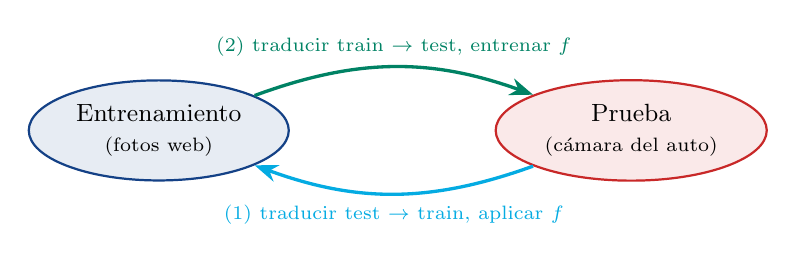
\begin{tikzpicture}[
				dom/.style={draw, thick, ellipse, minimum width=2.4cm, minimum height=1.2cm, align=center, font=\small},
				arr/.style={-Stealth, very thick}]
			\node[dom, draw=FixedBlue, fill=FixedBlue!10] (tr) at (0,0) {Entrenamiento\\ \scriptsize (fotos web)};
			\node[dom, draw=AdaptRed, fill=AdaptRed!10] (te) at (6,0) {Prueba\\ \scriptsize (c\'amara del auto)};
			\draw[arr, AccentGreen] (tr) to[bend left=20] node[above, font=\scriptsize] {(2) traducir train $\to$ test, entrenar $f$} (te);
			\draw[arr, UCMBlue] (te) to[bend left=20] node[below, font=\scriptsize] {(1) traducir test $\to$ train, aplicar $f$} (tr);
		\end{tikzpicture}
	\end{center}

	\vspace{0.2cm}

	\begin{block}{Estrategia}
		Hacer que ambas distribuciones sean \textbf{id\'enticas}: adaptar el dominio de prueba para que parezca el de entrenamiento, o viceversa.
	\end{block}

\end{frame}

\begin{frame}[shrink]{Adaptaci\'on de Dominio No Supervisada}

	\begin{block}{Datos Disponibles}
		\begin{itemize}
			\item Entrenamiento etiquetado: $\{(x^{(i)}, y^{(i)})\}_{i=1}^{N}$ del dominio fuente.
			\item Prueba \textbf{sin etiquetas}: $\{x'^{(j)}\}_{j=1}^{M}$ del dominio objetivo.
			\item No se pueden usar etiquetas de prueba, pero s\'i \textbf{alinear distribuciones}.
		\end{itemize}
	\end{block}

	\vspace{0.2cm}

	\begin{block}{Algoritmo: Traducci\'on Adversaria}
		\begin{enumerate}
			\item Entrenar un traductor $G$ (GAN, p.ej.\ CycleGAN) tal que $G(x)$ sea indistinguible de $x'$ para un discriminador $D$.
			\item Traducir el conjunto de entrenamiento: $\{(G(x^{(i)}), y^{(i)})\}$ (las etiquetas se conservan).
			\item Entrenar el clasificador $f$ sobre los datos traducidos.
			\item Aplicar $f$ directamente en el dominio de prueba.
		\end{enumerate}
	\end{block}

	\formula{
		\[
		\min_G \max_D \; \E_{x'}\big[\log D(x')\big] + \E_{x}\big[\log\big(1 - D(G(x))\big)\big]
		\]
	}

	\begin{alertblock}{Relaci\'on con Prompting}
		Ambos \textbf{editan la entrada}. Pero la adaptaci\'on de dominio busca alinear distribuciones (no optimizar la tarea) y no requiere acceso al modelo.
	\end{alertblock}

\end{frame}

% =================================================================
\section{Datos Generativos y Otros}

\begin{frame}[shrink]{Datos Generativos: Transferir la Distribuci\'on}

	Los datos sint\'eticos de un modelo generativo \textbf{no son s\'olo} una copia barata de datos reales.

	\vspace{0.3cm}

	\begin{columns}[T]
		\begin{column}{0.5\textwidth}
			\begin{block}{Cantidad}
				\small
				\begin{itemize}
					\item Muestras \textbf{ilimitadas}.
					\item Interpolan y remezclan los datos de entrenamiento de formas nuevas.
				\end{itemize}
			\end{block}
		\end{column}

		\begin{column}{0.5\textwidth}
			\begin{block}{Calidad}
				\small
				\begin{itemize}
					\item Cada muestra viene con su \textbf{procedimiento generativo}.
					\item Las variables latentes $z$ tienen estructura explotable.
				\end{itemize}
			\end{block}
		\end{column}
	\end{columns}

	\vspace{0.3cm}

	\begin{block}{Ejemplo: Vacas en la Playa}
		Un generador entrenado con im\'agenes al aire libre nunca vio vacas en la playa. \textbf{Editando $z$} se generan esas combinaciones y se entrena un clasificador robusto al contexto.
	\end{block}

	\vspace{0.2cm}

	\begin{alertblock}{Tipo de Conocimiento Transferido}
		Se transfiere conocimiento sobre la \textbf{distribuci\'on de los datos}, no una funci\'on aprendida: el clasificador final puede entrenarse desde cero.
	\end{alertblock}

\end{frame}

\begin{frame}{Otros Tipos de Conocimiento Transferible}

	Casi \textbf{cualquier componente} de un algoritmo de aprendizaje puede preentrenarse y transferirse.

	\vspace{0.3cm}

	\begin{columns}[T]
		\begin{column}{0.5\textwidth}
			\begin{block}{P\'erdida Aprendida}
				\small
				\begin{itemize}
					\item Preentrenar la propia funci\'on $\mathcal{L}$.
					\item Ej.: p\'erdidas perceptuales (LPIPS), discriminadores de GAN.
				\end{itemize}
			\end{block}
		\end{column}

		\begin{column}{0.5\textwidth}
			\begin{block}{Optimizador Aprendido}
				\small
				\begin{itemize}
					\item Preentrenar la regla de actualizaci\'on:
					\[
					\theta_{t+1} = \theta_t - g_\psi\big(\nabla_\theta \mathcal{L}, \ldots\big)
					\]
					\item $\psi$ se aprende sobre muchas tareas.
				\end{itemize}
			\end{block}
		\end{column}
	\end{columns}

	\vspace{0.4cm}

	\begin{alertblock}{Ejercicio Mental}
		Mire cada l\'inea del c\'odigo de entrenamiento (datos, modelo, p\'erdida, optimizador, inicializaci\'on) y preg\'untese: ¿esto podr\'ia preentrenarse?
	\end{alertblock}

\end{frame}

% =================================================================
\section{Cat\'alogo}

\begin{frame}{Un Cat\'alogo Combinatorio de M\'etodos}

	Todos los m\'etodos son \textbf{minimizaci\'on del riesgo emp\'irico}; difieren en \ad{qu\'e se adapta} y \fx{qu\'e queda fijo del preentrenamiento}.

	\vspace{0.3cm}

	\begin{center}
		\renewcommand{\arraystretch}{1.5}
		\begin{tabular}{lll}
			\toprule
			\textbf{M\'etodo} & \textbf{Objetivo de aprendizaje} & \textbf{Inferencia} \\
			\midrule
			Finetuning & $\arg\min_{\ad{\theta}} \E_{x,y}\big[\mathcal{L}(f_{\ad{\theta}}(x), y)\big]$, \ $\theta_0 = \fx{\theta}$ & $f_{\ad{\theta}}(x)$ \\
			Destilaci\'on & $\arg\min_{\ad{\theta}} \E_{x}\big[\mathcal{L}(f_{\ad{\theta}}(x), \fx{t}(x))\big]$ & $f_{\ad{\theta}}(x)$ \\
			Prompting & $\arg\min_{\ad{\epsilon}} \E_{x,y}\big[\mathcal{L}(f_{\fx{\theta}}(x \oplus \ad{\epsilon}), y)\big]$ & $f_{\fx{\theta}}(x \oplus \ad{\epsilon})$ \\
			Probes / heads & $\arg\min_{\ad{\phi}} \E_{x,y}\big[\mathcal{L}(h_{\ad{\phi}}(f_{\fx{\theta}}(x)), y)\big]$ & $h_{\ad{\phi}}(f_{\fx{\theta}}(x))$ \\
			P\'erdida aprendida & $\arg\min_{\ad{\theta}} \E_{x,y}\big[\fx{\mathcal{L}}(f_{\ad{\theta}}(x), y)\big]$ & $f_{\ad{\theta}}(x)$ \\
			Optimizador aprendido & $\fx{\arg\min}_{\ad{\theta}} \E_{x,y}\big[\mathcal{L}(f_{\ad{\theta}}(x), y)\big]$ & $f_{\ad{\theta}}(x)$ \\
			\bottomrule
		\end{tabular}
	\end{center}

	\vspace{0.2cm}

	\small \ad{Rojo}: se adapta en la nueva tarea. \quad \fx{Azul}: preentrenado y fijo. \quad (La adaptaci\'on de dominio no encaja limpiamente en este esquema.)

\end{frame}

\begin{frame}[shrink]{Una Caja de Herramientas, no una Lista}

	\begin{block}{Los M\'etodos se Combinan}
		\begin{itemize}
			\item Prompting + probe: tokens aprendidos y cabeza lineal sobre un ViT congelado.
			\item Destilaci\'on + finetuning: inicializar el estudiante con pesos preentrenados.
			\item LoRA + datos generativos: ajustar un modelo de difusi\'on y usarlo como fuente de datos.
		\end{itemize}
	\end{block}

	\vspace{0.3cm}

	\begin{block}{¿Qu\'e Elegir?}
		\small
		\begin{center}
			\renewcommand{\arraystretch}{1.3}
			\begin{tabular}{lccc}
				\toprule
				& \textbf{Par\'ametros nuevos} & \textbf{Acceso a pesos} & \textbf{Costo} \\
				\midrule
				Finetuning completo & todos & s\'i & alto \\
				LoRA / subpartes & pocos & s\'i & medio \\
				Probe lineal & muy pocos & s\'olo features & bajo \\
				Prompting & muy pocos & gradientes / caja negra & bajo \\
				Destilaci\'on & modelo nuevo & s\'olo salidas & medio \\
				\bottomrule
			\end{tabular}
		\end{center}
	\end{block}

\end{frame}

% =================================================================
\section{Modelos Secuenciales}

\begin{frame}{Modelos Secuenciales como Adaptaci\'on}

	Un modelo secuencial (RNN, Transformer) \textbf{cambia su comportamiento} seg\'un lo que ya ha visto: eso es adaptaci\'on en tiempo de ejecuci\'on.

	\vspace{0.3cm}

	\begin{center}
		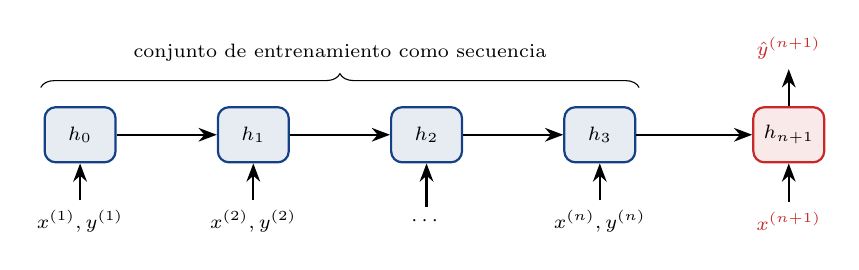
\begin{tikzpicture}[
				cell/.style={draw=UCMNavy, thick, fill=UCMNavy!10, rounded corners, minimum width=0.9cm, minimum height=0.7cm, font=\scriptsize},
				arr/.style={-Stealth, thick}]
			\foreach \i/\lab in {0/{x^{(1)},y^{(1)}}, 1/{x^{(2)},y^{(2)}}, 2/{\cdots}, 3/{x^{(n)},y^{(n)}}}{
				\node[cell] (h\i) at (2.2*\i,0) {$h_{\i}$};
				\node[font=\scriptsize] (in\i) at (2.2*\i,-1.1) {$\lab$};
				\draw[arr] (in\i) -- (h\i);
			}
			\foreach \i/\j in {0/1,1/2,2/3}{\draw[arr] (h\i) -- (h\j);}
			\node[cell, draw=AdaptRed, fill=AdaptRed!10] (q) at (9.0,0) {$h_{n+1}$};
			\node[font=\scriptsize, AdaptRed] (qx) at (9.0,-1.1) {$x^{(n+1)}$};
			\node[font=\scriptsize, AdaptRed] (qy) at (9.0,1.1) {$\hat{y}^{(n+1)}$};
			\draw[arr] (h3) -- (q); \draw[arr] (qx) -- (q); \draw[arr] (q) -- (qy);
			\draw[decorate, decoration={brace, amplitude=5pt}] (-0.5,0.6) -- (7.1,0.6) node[midway, above=6pt, font=\scriptsize] {conjunto de entrenamiento como secuencia};
		\end{tikzpicture}
	\end{center}

	\vspace{0.2cm}

	\begin{block}{Aprendizaje Supervisado con una RNN}
		\begin{itemize}
			\item Entrada: los pares de entrenamiento en orden $\{x^{(1)}, y^{(1)}, \ldots, x^{(n)}, y^{(n)}\}$.
			\item El estado oculto $h_n$ ``resume'' los datos: la funci\'on aprendida est\'a en $(\theta, h_n)$.
			\item Una consulta nueva $x^{(n+1)}$ produce $\hat{y}^{(n+1)}$ \textbf{sin ning\'un gradiente}.
		\end{itemize}
	\end{block}

\end{frame}

\begin{frame}[shrink]{Aprendizaje en Contexto y Metaaprendizaje}

	\begin{block}{Aprender = Adaptar el Comportamiento Futuro seg\'un Datos Pasados}
		\begin{itemize}
			\item Si entrenamos el modelo secuencial sobre \textbf{muchas tareas}, aprende a aprender: \textbf{metaaprendizaje}.
			\item En los grandes modelos de lenguaje esto emerge solo y se llama \textbf{aprendizaje en contexto} (\textit{in-context learning}).
		\end{itemize}
	\end{block}

	\vspace{0.3cm}

	\begin{center}
		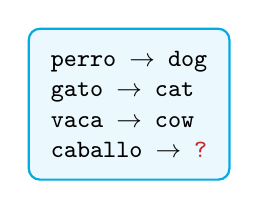
\begin{tikzpicture}[font=\small]
			\node[draw=UCMBlue, thick, rounded corners, fill=UCMBlue!8, align=left, inner sep=8pt] {
				\texttt{perro $\to$ dog}\\
				\texttt{gato $\to$ cat}\\
				\texttt{vaca $\to$ cow}\\
				\texttt{caballo $\to$ \textcolor{AdaptRed}{\textbf{?}}}
			};
		\end{tikzpicture}
	\end{center}

	\vspace{0.2cm}

	\begin{alertblock}{Significado}
		El ``aprendizaje'' emerge del modelado de secuencias, sin un procedimiento de entrenamiento expl\'icito. El prompt \textbf{es} el conjunto de entrenamiento.
	\end{alertblock}

\end{frame}

% =================================================================
\section{Conclusiones}

\begin{frame}{Conclusiones y Perspectivas}

	\begin{itemize}
		\item \textbf{Preentrenar + adaptar} es el paradigma dominante: casi nadie entrena desde cero.

		\vspace{0.25cm}

		\item Lo que se transfiere puede ser:
		\begin{itemize}
			\item \textbf{Pesos} $\to$ finetuning, LoRA, probes lineales.
			\item \textbf{Salidas} $\to$ destilaci\'on de conocimiento.
			\item \textbf{Entradas} $\to$ prompting, adaptaci\'on de dominio.
			\item \textbf{Datos} $\to$ modelos generativos como fuente de entrenamiento.
		\end{itemize}

		\vspace{0.25cm}

		\item Los m\'etodos son \textbf{combinables}: una caja de herramientas sobre la misma minimizaci\'on del riesgo emp\'irico.

		\vspace{0.25cm}

		\item Los modelos secuenciales muestran que la adaptaci\'on puede ocurrir \textbf{sin gradientes} (aprendizaje en contexto).

		\vspace{0.25cm}

		\item Mientras no existan modelos universales \textit{zero-shot}, la adaptaci\'on seguir\'a siendo esencial, y su importancia crece con la escala de los modelos.
	\end{itemize}

	\vspace{0.2cm}

	{\scriptsize Fuente: Torralba, Isola \& Freeman, \textit{Foundations of Computer Vision}, cap.\ 37 (visionbook.mit.edu).}

\end{frame}

\end{document}
